\begin{section}{SC}{A Cosmic Web Filament Revealed in Lyman-α Emission around \\
    \hspace*{4cm} a Luminous High-Redshift Quasar}{(Prof. Sebastiano Cantalupo)}
  \begin{minipage}{\linewidth}
    \begin{wrapfigure}{r}{0pt}
      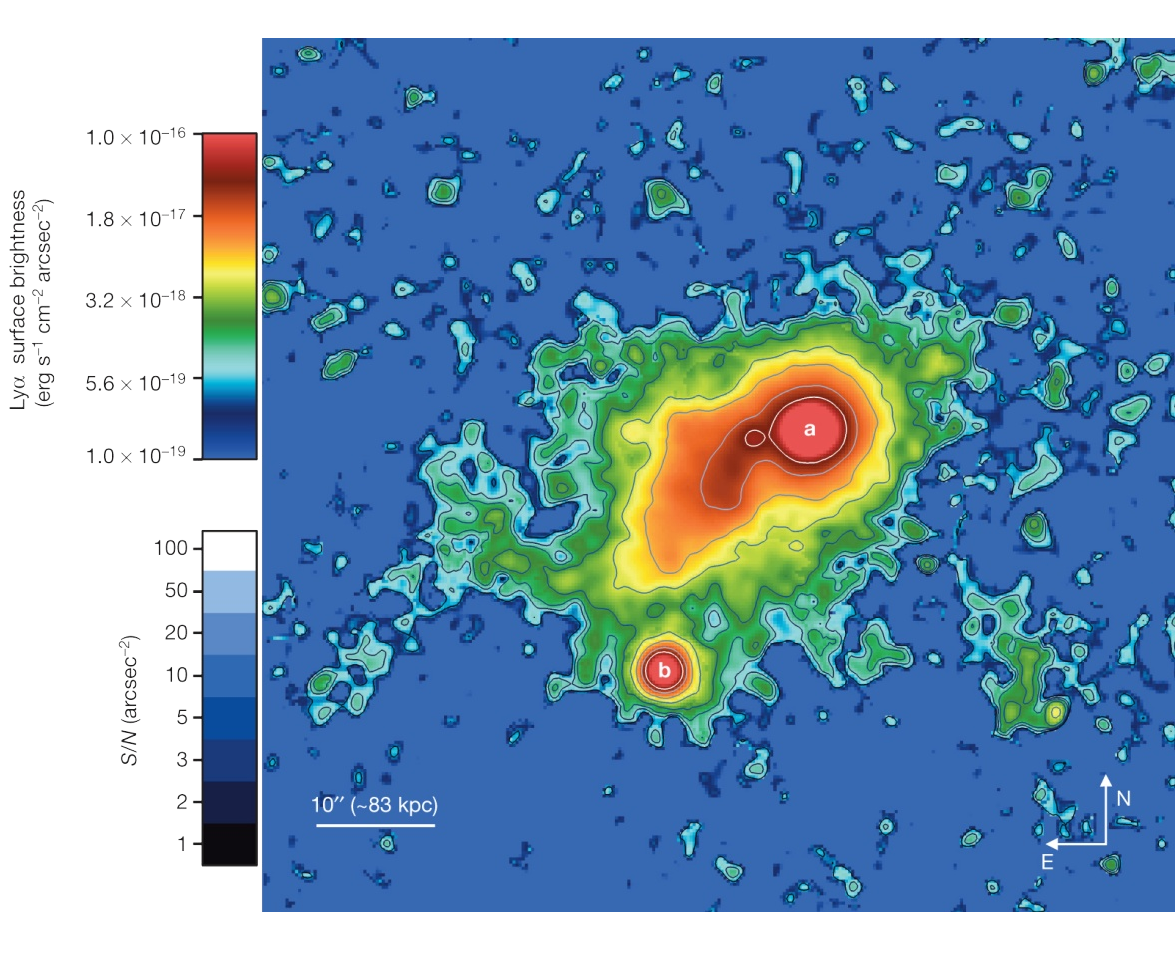
\includegraphics[height=13cm]{SC/Slug.png}
    \end{wrapfigure}
    \strut {\small Simulations of structure formation in the Universe
      predict that galaxies are embedded in a ‘cosmic web’1, where most
      baryons reside as rarefied and highly ionized gas2. This material has
      been studied for decades in absorption against background sources3,
      but the sparseness of these inherently one-dimensional probes preclude
      direct constraints on the three-dimensional morphology of the
      underlying web. Here we report observations of a cosmic web filament
      in Lyman-α emission, discovered during a survey for cosmic gas
      fluorescently illuminated by bright quasars4, 5 at redshift z ≈ 2.3.
      With a linear projected size of approximately 460 physical
      kiloparsecs, the Lyman-α emission surrounding the radio-quiet quasar
      UM 287 extends well beyond the virial radius of any plausible
      associated dark-matter halo and therefore traces intergalactic gas.
      The estimated cold gas mass of the filament from the observed
      emission—about 1012.0 ± 0.5/C1/2 solar masses, where C is the gas
      clumping factor—is more than ten times larger than what is typically
      found in cosmological simulations5, 6, suggesting that a population of
      intergalactic gas clumps with subkiloparsec sizes may be missing in
      current numerical models.}
  \end{minipage}

  \vspace{0.7cm}

  {\footnotesize \textit{[Cantalupo et al. 2017, 2014Natur.506...63C]}}
\end{section}